\documentclass{article}

\usepackage{mystyle}

\setenumerate[0]{label=(\alph*)} % Set default of enumerate to be alphabetical
\graphicspath{ {./img/} } % path to image folder

\begin{document}
v
\maketitle

\newpage

\tableofcontents

\newpage

\section{Recurrent Models for MNIST}

\subsection{Understanding LSTM vs GRU}

We specify the LSTM and GRU cells and recurrence equations.

\begin{description}
\item[LSTM]

  \begin{align}
    f_t & = \sigma_g (W_f x_t + U_f h_{t-1} + b_f) \\
    i_t & = \sigma_g (W_i x_t + U_i h_{t-1} + b_i) \\
    o_t & = \sigma_g (W_o x_t + U_o h_{t-1} + b_o) \\
    c_t & = f_t \odot c_{t-1} + i_t \odot \sigma_g(W_c x_t + U_c h_{t-1} + b_c) \\
    h_t & = o_t \odot \tanh (c_t)
  \end{align}

  where $\sigma_g$ is the sigmoid activation function.
  
\item[GRU]

  \begin{align}
    z_t & = \sigma_g (W_z x_t + U_z h_{t-1} + b_z) \\
    r_t & = \sigma_g (W_r x_t + U_r h_{t-1} + b_r) \\
    h & = \tanh(W_h x_t + U_f (h_{t-1} \odot r_t) + b_h) \\
    h_t & = (1 - z_t) \odot h + z_t \odot h_{t-1}
  \end{align}

  We also note that any composition of affine transformations and the sigmoid
  functions in these cases never lead to inverses of the sigmoid functions, and only the case
  of $\sigma(constant)$ leads to linearity.
    
\end{description}

\begin{enumerate}   
\item

  Reframing the question: define the LSTM cell to be a function $h_t =
  g_{\Theta}(x_{t})$, where $\Theta$ are all of the parameters of the LSTM
  cell, $\{W, U, b\}_{f, i, o, c}$. Similarly for the GRU cell. We are trying to
  find parameters that in general make the equivalence

  \begin{equation}
    h_t = x_{t} = g_{\Theta}(x_{t})
  \end{equation}

  true. Since this implies that $g_{\Theta} = Id$ which is linear, linearity is
  a necessary condition for this to be true. Hence if we can show that linearity
  doesn't hold in general, or that the only linear case is independent of $x_t$
  (i.e. constant with regards to $x_t$) then this also implies that $h_t \neq x_{t}$ in
  general.

    \begin{description}
  \item[LSTM] We consider $g_{\Theta} =: g$ and try to find $\Theta$ that makes
    $g$ linear. Since

    \begin{align*}
      h_t = o_t \odot \sigma_h( c_t )
    \end{align*}

    We need both $o_t$ and $\sigma_h( c_t )$ to be linear in $x_t$. This in turn
    implies that $c_t$ is constant with respect to $x_t$ since else the whole
    thing is non-linear. Similarly as

    \begin{equation*}
      o_t = \sigma_g (W_o x_t + U_o h_{t-1} + b_o)
    \end{equation*}

    we need this to be constant in $x_t$ as else it is non-linear. But this
    means that both $o_t, c_t$ are constant with respect to $x_t$ which implies
    that $h_t$ doesn't depend on $x_t$, which means that $g_{\Theta}$ can't be the
    identity function of $x_t$. So we have shown that this is not possible for
    LSTM.

    However, if we take the limit case where the sigmoid function can take on
    the values 0 and 1, and $\tanh$ the values -1 and 1 (done by letting the
    bias term $b$ go to $\pm \infty$ elementwise to the same limit), we can 'store' the
    input value $x_t$ but only through the non-linear layer. This can be done by
    setting $W_o = I, U_o = 0, b_o = 0$, and $f_t, i_t = 0$ by letting $b_i, b_f
    \to - \infty$, then $h_t = \sigma(x_t)$. In general we have a map from two
    spaces which are of different dimensions, so an identity in this case is not
    possible.
    
  \item[GRU] Similarly as to the LSTM we have the relation

    \begin{equation*}
      h_t = g_{\Theta}(x_t) = (1 - z_t) \odot h + z_t \odot h_{t-1}
    \end{equation*}

    reasoning as in the case with LSTM, we need both terms of the addition to be
    linear, the necessary condition. We have the two terms $(1 - z_t) \odot h$
    and $z_t \odot h_{t-1}$. Since $z_t$ is a non-linear function in $x_t$ or
    constant in $x_t$ and $h_{t-1}$ is independent of $x_t$ we must be able to
    kill off the terms that lead to a non-linear function in $x_t$. We see that
    since $h_{t_1}$ is given and assumed equal to $x_{t-1}$ that $z_t = 0$ which
    implies that we must have

    \begin{equation*}
      h_t = h = \tanh(W_h x_t + U_f (h_{t-1} \odot r_t) + b_h)
    \end{equation*}

    But this is either constant or non-linear in $x_t$ hence it can't the be
    identity function. So we have shown that this is not possible for GRU.

    Interpreting storing as in $h_t$ only depending on $x_t$, we can do that by
    letting $z_t = 0$ by letting $b_z \to -\infty$ setting $W_z, U_z = 0$ and
    setting $U_h, b_h = 0, W_h = I$, meaning that $h_t = \tanh(x_t)$. 
    
  \end{description}
  
\item

  \begin{description}
  \item[LSTM]

    We want to show that there is a configuration such that $c_t = c_{t - 1}$.
    This is simply done by setting $i_t = 0, f_t = 1$ by letting $W_i, U_i = 0,
    b_i \to -\infty$ and $W_f, U_f = 0, b_f \to \infty$.
    
  \item[GRU]

    For the GRU we can make $h_t = h_{t-1}$ by setting the $z_t = 1$ by letting
    $W_z, U_z = 0, b_z \to \infty$. Then $h_t = 0 \odot h + h_{t-1} = h_{t-1}$.
    
  \end{description}

\item We define a shorthand for the notation of an affine transformation as

  \begin{equation*}
    A_l(x_t, h_{t-1}) = W_l x_t + U_l h_{t-1} + b_l
  \end{equation*}

  With this we note that we can decompose the output and state for the LSTM and
  GRU as

  \begin{description}
  \item[LSTM]

    \begin{align*}
      h_t & = \sigma(A_o(x_t, h_{t-1})) \odot \\
          & (\sigma(\sigma(A_f(x_t, h_{t-1})) \odot c_{t-1} + \sigma(A_i(x_t, h_{t-1})) \odot \tanh(A_c(x_t, h_{t-1})))) \\
          & = \sigma(A_o(x_t, h_{t-1})) \odot \sigma(\sigma(A_f(x_t, h_{t-1})) \odot c_{t-1} + \sigma(A_i(x_t, h_{t-1})) \odot \tanh(A_c(x_t, h_{t-1}))))
    \end{align*}
    
  \item[GRU]

    \begin{align*}
      h_t & = \tanh(A_h(x_t, h_{t-1} \odot \sigma(A_r(x_t, h_{t-1})))) \\
          & - \tanh(A_h(x_t, h_{t-1} \odot \sigma(A_r(x_t, h_{t-1})))) \odot \sigma(A_z(x_t, h_{t-1})) \\
          & + \sigma(A_z(x_t, h_{t-1})) \odot h_{t-1}
    \end{align*}

    We now construct a counter-example showing that the GRU is not a special
    case of the LSTM. Consider the scalar case. Let $A_z$ be zero, $A_h$ be such
    that $W_h = 1, U_h = 1, b_h = 1$, equally for $A_r$. This gives us that

    \begin{equation*}
      h_t = 0.5\tanh(x_t + h_{t-1}\sigma(x_t + h_{t-1} + 1) + 1) + 0.5 h_{t-1}
    \end{equation*}

    We see that the LSTM can never have this form since we have a sigmoid
    function inside of the $\tanh$ function which doesn't exist for the LSTM.
    Thus the GRU is not in general a special case of the LSTM.
    
  \end{description}

\end{enumerate}

\section{Task 1: Classification}

For task 1 I implemented a python file called \texttt{task1.py}. By design you
pass to this function several command line arguments which lets you pick the
architectures that we are interested in. The differences in all of the models
have to do with either the cell type used in the RNN part of the network (LSTM
or GRU) or the innards of the cell (32, 64, 128 or 3 stacks of 32 for the hidden
unit). Finally we also have to fix the first part of the output network (the
feed forward part of the whole architectures) since it has to map the output to
the assumed 100 dimensions after the first layer. Since my design takes all
models into consideration, what I will describe below applies to all models of
task 1. All of this was done using the functions in tensorflow, and this was
done for all architectures and models in this assignment.

The models mainly differ in their expressive power, since a higher number of
hidden units in the RNN gives a bigger space of functions that the whole network
can represent it should be able to learn more aspects of the data set. However
this also means that it should be easier to overfit. The stacked layer network
is somewhere in between, but should possibly be the most expressive of them all
since the parameters of each layer are independent in a way that the 128 hidden
units model is not.

\subsection{Architecture}

My architecture is straightforward, the only difference between the vanilla
implementation in the notes is that for the feed forward layers, I use batch
normalisation.

I used batch normalisation since this reduces the internal covariate shift at
each layer. Essentially, models are able to learn patterns much better if the
input distribution of each layer is the same during training. For deep models it is common that
as we use backpropagation and change the parameters of the shallow layers, the
distribution of the input of the deeper layers change. Batch normalisation
mitigates this by normalising the input. In our case, I used batch normalisation
before the input to the affine layers in the final part of the network, the
feed-forward network following the recurrent neural network part. Thus my
architecture includes two instances of batch normalisation, once directly after
the output from the RNN and once after the first non-linearity in the
feed-forward network.

Batch normalisation is different during training and testing as during
training the normalisation is done with respect to batch mean and variance of
the layer input which is dependent on how you batch your data set during
training, while for testing these parameters are fixed. To get estimates of the
population mean and variance of each layer input to be used during testing I
kept an exponential running average of the mean and variance.

Define the index $i$ to show belonging to layer $i$ and letting $t$ denote the
time step of training, $B_t$ the batch at time $t$. The input to layer $i$ will
have some distribution. This distribution will when we are finished with
training have some population mean and variance $\mu^i, \sigma^{2i}$. We then estimate
these parameters to be used during test time by keeping an exponential running
average. That is, if at time $t$ we have the batch estimates of the parameters
$\mu^i_{t, B}, \sigma^{2i}_{B, t}$ then we update the estimates of the population
parameters, $\hat{\mu}^i_t, \hat{\sigma}^{2i}_t$ with a chosen decay rate $d$ as 

\begin{align*}
  \hat{\mu}^i_t & = d * \hat{\mu}^i_{t-1} + (1 - d) * \mu^i_{t, B} \\
  \hat{\sigma}^{2i}_t & = d * \hat{\sigma}^{2i}_{t-1} + (1 - d) * \sigma^{2i}_{t, B} \\
\end{align*}

where we initialise the running averages to be

\begin{align*}
  \hat{\mu}^i_0 & = 0 \\
  \hat{\sigma}^{2i}_0 & = 1 
\end{align*}

The decay rate specifies how much we take previous data into consideration and
gives us a more accurate estimate given that we train long enough so that we
forget the initialisations.

Running the training for a long enough time enables us to get accurate estimates
of the population mean and variance. Note that in general these parameters are
vectors.

During train time the batch normalisation then applies the operation to each
input of batch $B$ of layer $i$ as

\begin{equation}
  BN_{\gamma, \beta}(x^i) = \gamma * \frac{x^i - \mu^i_B}{\sigma^i_B} + \beta
\end{equation}

where $\gamma$ and $\beta$ are vectors to be learned. This also has a
regularising effect meaning that we don't have to rely on dropout to reduce
overfit.\footnote{https://arxiv.org/abs/1502.03167}

Similarly is done during test, except that we know use the estimated mean and
variance instead of the batch mean and variance.

The batch normalisation helps a lot, without the training is highly erratic and
often resets to random prediction in terms of loss and accuracy. With batch
normalisation I am able to reach much better results, in a shorter number of
training steps, which reinforces the results of the paper.\footnote{https://arxiv.org/abs/1502.03167}

\subsection{Hyperparameters and optmization}

Before I used batch normalisation I had a hard time getting the models to train
properly. After experimenting I found that ADAM seemed to yield the best
training performance, both with and without batch normalisation. As ADAM is a
pretty advanced optimisation algorithm which has been shown to work well on
training neural networks this is no surprise as it takes into account more of
the aspects of the trajectory than just SGD which just looks at the current
position to calculate the next one given the learning rate and batch through the
derivatives gotten from the backpropagation.

Since batch normalisation yields models which train in a much more stable manner
than without it as it reduces internal covariate shift I was able to
consistently get great results by using the hyperparameters of

\begin{description}
\item[learning rate] 0.001
\item[decay rate] 0.99
\item[batch size] 256
\end{description}

This was the same for all models except for GRU with 32 hidden units of 3 layers
as my computer died that I had running at home, and rerun it with 60 epochs instead.

The learning rate enables training the models until saturation and they achieved
consistently increasing accuracy except for possibly 3 stacked hidden layers of
32 units each, but I am not sure if this should be the case or not since it
doesn't seem clear to me if this yields a more or less flexible model compared
to one hidden layer of size 128. Also, since using batch normalisation means
that good results can be achieved for a bigger set of hyperparameters, I did not
need to search as many alternative triplets of hyperparameters as if I had
trained without batch normalisation. There is also some indication that even 100
epochs was not enough for this model to fully converge.

The decay rate doesn't really impact accuracy except for that we need the final
estimates of the mean and variance of the batch normalisation operators in the
neural networks to be accurate estimates of the population parameters for these
layers. This is independent of the back propagation and just means that we need the
number of training steps to be large enough so that the resulting estimated
means and variances are able to 'forget' the starting values of these
parameters. Since I trained for 100 epochs which means I did approximately 21500
training steps, 0.99 should be small enough to get away from the
initialisations, but high enough to yield correct estimates.

The batch size was chosen to be reasonably big to exploit both the fact that
tensorflow uses highly optimized linear algebra packages which
means that we get significant speedups by processing in big batches rather than
increasing the number of iterations in the train loops, but small enough such
that it still is stochastic and can climb out of local minima. Since I trained
my models using GPU instances on AWS, The batch size
was deliberately chosen to be a multiple of 32 since this meant I could optimize
the use of the GPU cache and avoid cache misses speeding up training.

I trained for each model for 100 epochs. At the end of each epoch I recorded the
test and train accuracy and loss, using random batches of the train and test set
of size 800. Using the test accuracy I saved the model every time the test
accuracy increased compared to all the previous test accuracies during that run.
This amounts to a kind of early stopping. Since I used the test set to set
hyperparameters I might overfit, however, since the accuracies were stochastic
this mitigates this somehow. Nevertheless I believe that the result should
generalise well.

\subsubsection{Graphs}

We have the following graphs from training the models in task 1.\footnote{These images are
sufficient to get a good overview of the training. However, they are easier to
interpret interactively by running \texttt{tensorboard
  --logdir=./models} from the parent directory and then going to the
link using Chrome.} Note that the filled trajectories are smoothed with a
smoothing value of 0.5 in tensorboard, while the shadow trajectories are the
original trajectories without smoothing.

\textbf{LSTM}

\begin{figure}[H]
  \centering
  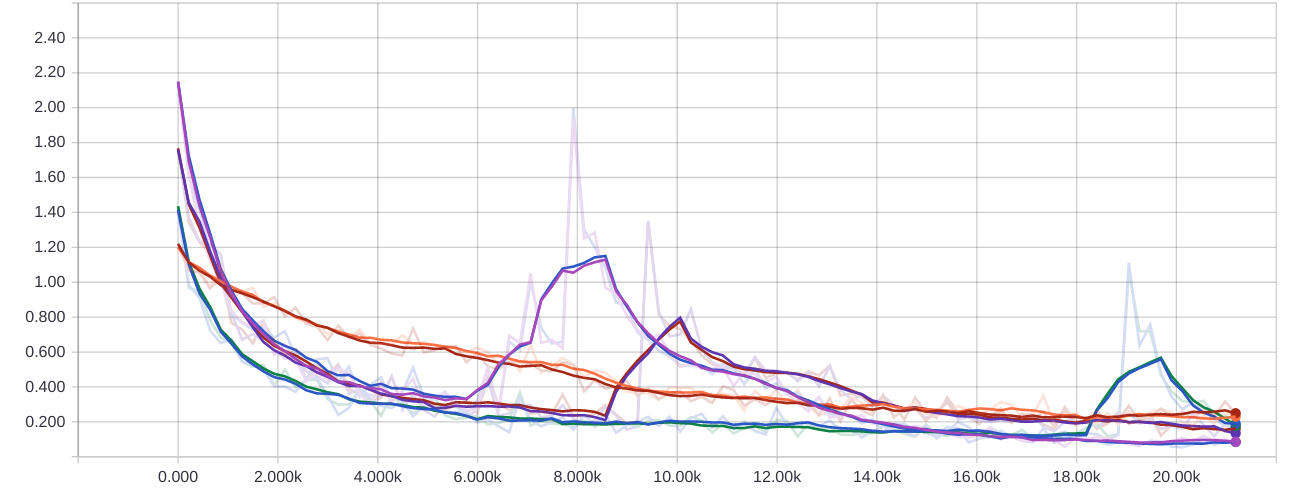
\includegraphics[width=0.8\textwidth]{task1/LSTM_task1_loss.png}
  \caption{Cross entropy vs training steps}
  \label{fig:LSTM_Xent_1}
\end{figure}

\begin{figure}[H]
  \centering
  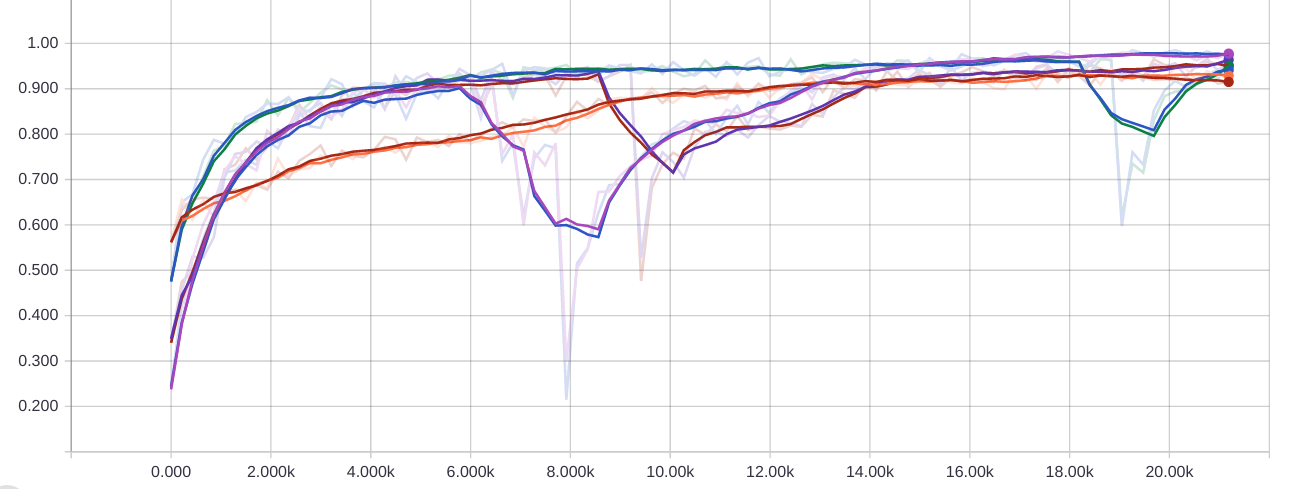
\includegraphics[width=0.8\textwidth]{task1/LSTM_task1_acc.png}
  \caption{Accuracy vs training steps}
  \label{fig:LSTM_acc_1}
\end{figure}

\textbf{Legend}. I will list them pairwise from the lowest starting point in the accuracy
graph to the highest (opposite for the graph of the loss). The first colour is the train set, second colour the test set:

\begin{description}
\item[Blue/Purple] 128 hidden units
\item[Red/Dark Purple] 64 hidden units
\item[Green/Blue] 3 stacked layers of 32 hidden units
\item[Orange/Red] 32 hidden units
\end{description}

\textbf{GRU}

\begin{figure}[H]
  \centering
  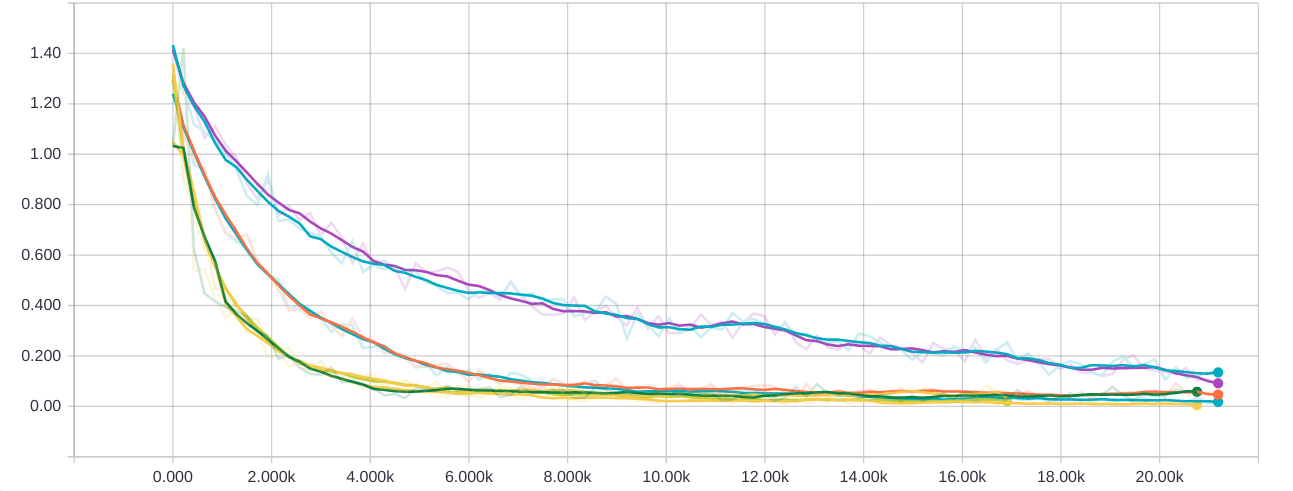
\includegraphics[width=0.8\textwidth]{task1/GRU_task1_loss.png}
  \caption{Cross entropy vs training steps}
  \label{fig:GRU_Xent_1}
\end{figure}

\begin{figure}[H]
  \centering
  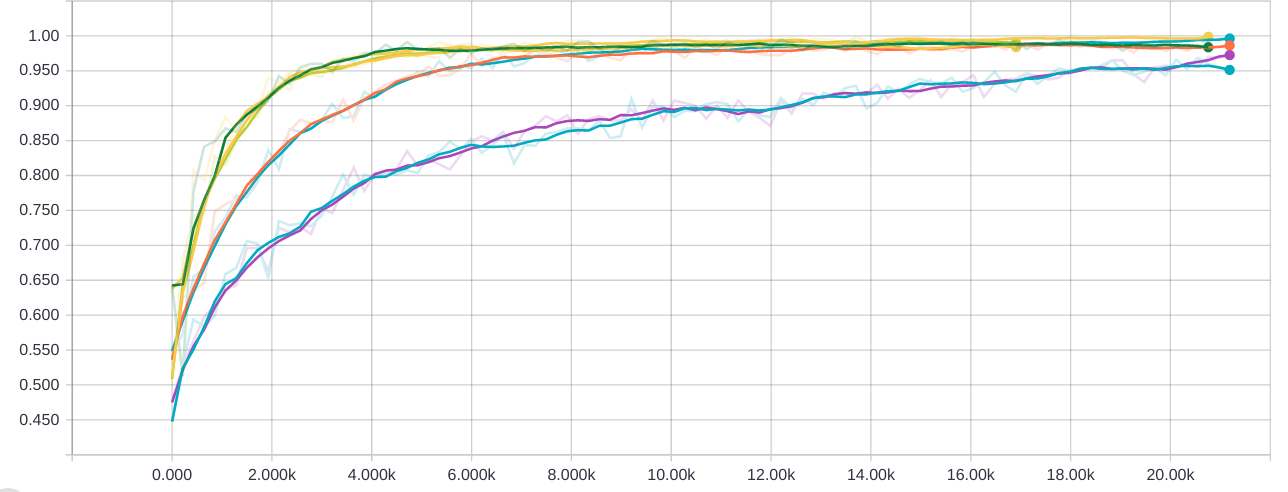
\includegraphics[width=0.8\textwidth]{task1/GRU_task1_acc.png}
  \caption{Accuracy vs training steps}
  \label{fig:GRU_acc_1}
\end{figure}

\textbf{Legend}. I will list them pairwise from the lowest starting point in the accuracy
graph to the highest (opposite for the graph of the loss). The first colour is the train set, second colour the test set:

\begin{description}
\item[Dark Purple/Cyan] 32 hidden units
\item[Gold/Yellow] 64 hidden units
\item[Purple/Cyan] 3 stacked layers of 32 hidden units
\item[Green/Yellow] 128 hidden units
\end{description}

Comparing these graphs for LSTM and GRU, we see that while both seem to converge
over enough epochs, the 
GRU's have a much more stable training than the LSTM's, and much better end
results as can bee seen in the results section.. Naturally the results
will fluctuate somehow, and since I take stochastic estimations of accuracy and
loss at the end of each epoch, this is not surprising. However, I did not think
that there would be such a massive difference as we can see from the graphs. If
we look at the shadow trajectories of the LSTM's we note that several of the
trajectories drop from a good result down to almost baseline accuracy/loss. This
influenced my decision to use GRU's in task 2 since they seem better fit to the
task. I don't know if this can be generalised beyond these architectures/data
set.

From the graph we can see that there is an improvement in the accuracy/loss as
the number of hidden units increases, but the 3 stacked layers of 32 hidden
unit cells falls in between, possibly as it converges much more slowly than the
rest. However, in order to conclude this we should collect data over several
runs to make sure that this i not a statistical fluke.

\subsection{Results}

\begin{center}
  \begin{tabular}{ |c|c|c|c|c| } 
    \hline
    Model: LSTM & (1 layer, 32 units) & (1 layer, 64 units) & (1 layer, 128 units) & (3 layers, 32 units) \\
    \hline
    Testing Loss & 0.25888 & 0.20495 & 0.23591 & 0.46100 \\
    Training Loss & 0.26707 & 0.19597 & 0.24081 & 0.45192 \\
    \hline
    Testing Accuracy & 0.92130 & 0.94180 & 0.93150 & 0.85900 \\
    Training Accuracy & 0.91827 & 0.94342 & 0.93053 & 0.86185 \\
    \hline
  \end{tabular}
\end{center}

\begin{center}
  \begin{tabular}{ |c|c|c|c|c| } 
    \hline
    Model: GRU & (1 layer, 32 units) & (1 layer, 64 units) & (1 layer, 128 units) & (3 layers, 32 units) \\
    \hline
    Testing Loss & 0.15829 & 0.05887 & 0.05793 & 0.08601 \\
    Training Loss & 0.16102 & 0.03587 & 0.03767 & 0.06462 \\
    \hline
    Testing Accuracy & 0.95240 & 0.98310 & 0.98180 & 0.97550 \\
    Training Accuracy & 0.95136 & 0.98796 & 0.98709 & 0.97975 \\
    \hline
  \end{tabular}
\end{center}

Comparing this to the result in assignment one we get that these are slightly
worse in general than the network which saw the whole image at once. This is to
be expected since even though RNN's have a way to store previous information in
the input sequence, it still can't see the whole image at once and get a
holistic overview like in assignment 1. However, I think if I used batch
normalisation in assignment 1 and 2 compared to just in assignment 2 here, the
differences would be more pronounced.

\section{Task 2: Pixel prediction}

Similarly to task 1 I made the python file \texttt{task2a.py} able to train all
the different models (32, 64, 128, 3 stacks of 32) by choosing arguments from
the command line. I chose the GRU's since my experiments and plots from task 1
showed me that GRU's gave a higher accuracy for both training and test set and a
much more consistent training trace than LSTM's which was more choppy and
occasionally well into training dropped back to a performance equivalent to
random initialization. Additionally, this suggests that LSTM's are much more
prone to destroying the learned patterns when ADAM updates the parameters than
the GRU cell.

The same analysis as in task 1 applies here:

The models mainly differ in their expressive power, since a higher number of
hidden units in the RNN gives a bigger space of functions that the whole network
can represent it should be able to learn more aspects of the data set. However
this also means that it should be easier to overfit. The stacked layer network
is somewhere in between, but should possibly be the most expressive of them all
since the parameters of each layer are independent in a way that the 128 hidden
units model is not.

\subsection{Architecture}

The architecture is very similar to that of Task 1. The difference is that
instead of using the many-to-one RNN as in task 1 we are using a many-to-many
architecture. This is done by getting the output at each point and running it
through an affine layer which maps it down from the number of hidden units to a
scalar which is then squashed, equivalent to logistic regression. This number is
then interpreted as the probability of the next pixel being filled in. Using
this probability vector where the $i$'th entry corresponds to the probability
over the $i+1$'th pixel, we can use the original input vector as our output
vector by slicing it from the second to the last element. This lets us calculate
the average cross entropy per pixel which we can use backpropagation on to learn
the optimal parameters of the model.

I didn't use any batch normalisation in task 2 since it worked fine without it.

\subsection{Hyperparameters}

The hyperparameters chosen mimics that of task 1. I ran the models for 50 epochs
since they converged much faster than in task 1.

We have the following hyperparameters for all of the models

\begin{description}
\item[learning rate] 0.001
\item[batch size] 256
\end{description}

The hyperparameters were chosen for the same reason as in task 1. A 0.001
learning rate worked perfect for all models and gave a smooth trajectory and
good final performance. I saved the models every time the test accuracy went
below the best accuracy so far for each epoch. This possibly meant I overfit,
but it looks like it will give good generalisation performance.

The batch size was chosen to be big enough to take advantage of the
vectorisation and GPU's on AWS but small enough to be a source of stochasticity
meaning that we don't get stuck in local minima as easily.

\subsubsection{Graphs}

We have the following graphs from training the models in task 2.\footnote{These images are
sufficient to get a good overview of the training. However, they are easier to
interpret interactively by running \texttt{tensorboard
  --logdir=./models} from the parent directory and then going to the
link using Chrome.} Note that the filled trajectories are smoothed with a
smoothing value of 0.5 in tensorboard, while the shadow trajectories are the
original trajectories without smoothing.

\begin{figure}[H]
  \centering
  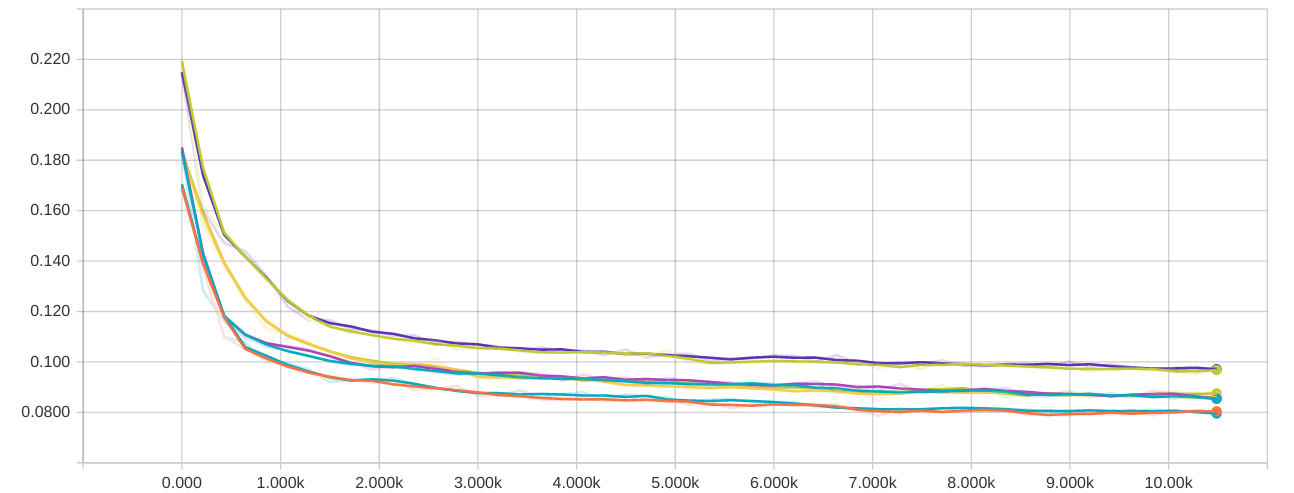
\includegraphics[width=0.8\textwidth]{task2/GRU_task2_loss.png}
  \caption{Cross entropy vs training steps (GRU)}
  \label{fig:GRU_Xent_2}
\end{figure}

\begin{figure}[H]
  \centering
  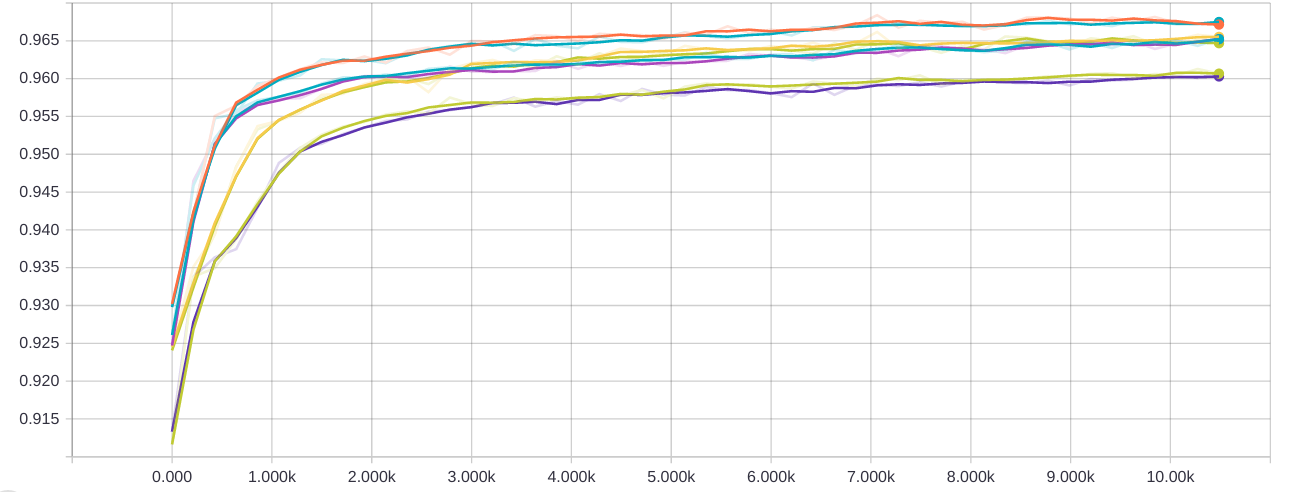
\includegraphics[width=0.8\textwidth]{task2/GRU_task2_acc.png}
  \caption{Accuracy vs training steps (GRU)}
  \label{fig:GRU_acc_2}
\end{figure}

\textbf{Legend}. I will list them pairwise from the lowest starting point in the accuracy
graph to the highest (opposite for the graph of the loss). The first colour is the train set, second colour the test set:

\begin{description}
\item[Dark Purple/Gold] 32 hidden units
\item[Gold/Yellow] 64 hidden units
\item[Purple/Cyan] 3 stacked layers of 32 hidden units
\item[Cyan/Orange] 128 hidden units
\end{description}

Conclusion about the performance of the different models mirror the conclusions
of task 1.

\subsection{Results}

\begin{center}
  \begin{tabular}{ |c|c|c|c|c| } 
    \hline
    Model: GRU & (1 layer, 32 units) & (1 layer, 64 units) & (1 layer, 128 units) & (3 layers, 32 units) \\
    \hline
    Testing Loss & 0.09659 & 0.08784 & 0.08092 & 0.08532 \\
    Training Loss & 0.09744 & 0.08867 & 0.08154 & 0.08610 \\
    \hline
  \end{tabular}
\end{center}

\subsection{Cross-entropies}

Using the code as specified in \texttt{task2b.py} we calculate the average
per-pixel cross-entropy averaged over the 10 generated inpaintings of the set of
100 masked images from the test set (The normal cross entropy, ground truth or
inpaintings, for one image is reported as an average over the inpainted masked
pixels, we then produce 1000 images, 10 generated samples per image sampled from
the test set. Finally we average the pixel cross-entropy over all of the
100*10=1000 images).

\subsubsection{Tables}

\begin{center}
  \begin{tabular}{ |c|c|c| } 
    \hline
    GRU 32 & Ground Truth & Inpaintings \\
    \hline
    1 pixel & 0.17033 & 0.14874 \\
    10 pixels & 0.38597 & 0.20815 \\
    28 pixels & 0.21755 & 0.12829 \\
    300 pixels & 0.79950 & 0.09417 \\
    \hline
  \end{tabular}
\end{center}

\begin{center}
  \begin{tabular}{ |c|c|c| } 
    \hline
    GRU 64 & Ground Truth & Inpaintings \\
    \hline
    1 pixel & 0.16718 & 0.17623 \\
    10 pixels & 0.35977 & 0.19590 \\
    28 pixels & 0.20932 & 0.12678 \\
    300 pixels & 0.60323 & 0.07297 \\
    \hline
  \end{tabular}
\end{center}

\begin{center}
  \begin{tabular}{ |c|c|c| } 
    \hline
    GRU 128 & Ground Truth & Inpaintings \\
    \hline
    1 pixel & 0.16667 & 0.13610 \\
    10 pixels & 0.29943 & 0.18597 \\
    28 pixels & 0.18047 & 0.12209\\
    300 pixels & 0.53247 & 0.06623 \\
    \hline
  \end{tabular}
\end{center}

\begin{center}
  \begin{tabular}{ |c|c|c| } 
    \hline
    GRU 3 stacked 32 & Ground Truth & Inpaintings \\
    \hline
    1 pixel & 0.15753 & 0.17612 \\
    10 pixels & 0.36390 & 0.18387 \\
    28 pixels & 0.20713 & 0.11607 \\
    300 pixels & 0.69276 & 0.07297 \\
    \hline
  \end{tabular}
\end{center}

\subsubsection{Comparison of the models}

We have the same kind of comparison as in task 1. Due to the increased
expressive power, as we trained the 

\subsection{Interesting inpaintings}

% What images to pick for 1. correct, 2. wrong, 3. high variance
\newcommand\digitA{33}
\newcommand\digitB{65}
\newcommand\digitC{77}

For the inpaintings I observed that numbers which are distinct (1, 4, 0) were more often
filled in correctly than numbers which are ambiguous (2, 3, 5, 6, 8, 9).
However, we have an additional source of noise since the binarization sometimes
leave us with ambiguous representations of the original image due to how it
thresholds.

All the images are arranged such that from left to right we have

\begin{enumerate}[label=\arabic*.]
\item Original image
\item Masked image
\item Sample 1
\item Sample 2
\item Sample 3
\item Sample 4
\item Sample 5
\end{enumerate}

\subsubsection{10 pixels inpaintings}

\begin{figure}[H]
  \centering
  \subfloat[32 GRU]{
    \includegraphics[scale=0.9]{task2/task2b32pixels10/images/index_\digitA.png}
  }
  \hspace{0mm}
  \subfloat[64 GRU]{
    \includegraphics[scale=0.9]{task2/task2b64pixels10/images/index_\digitA.png}
  }
  \hspace{0mm}
  \subfloat[128 GRU]{
    \includegraphics[scale=0.9]{task2/task2b128pixels10/images/index_\digitA.png}
  }
  \hspace{0mm}
  \subfloat[3 stack 32 GRU]{
    \includegraphics[scale=0.9]{task2/task2b32st3pixels10/images/index_\digitA.png}
  }
  \caption{Digit A}
\end{figure}

\begin{figure}[H]
  \centering
  \subfloat[32 GRU]{
    \includegraphics[scale=0.9]{task2/task2b32pixels10/images/index_\digitB.png}
  }
  \hspace{0mm}
  \subfloat[64 GRU]{
    \includegraphics[scale=0.9]{task2/task2b64pixels10/images/index_\digitB.png}
  }
  \hspace{0mm}
  \subfloat[128 GRU]{
    \includegraphics[scale=0.9]{task2/task2b128pixels10/images/index_\digitB.png}
  }
  \hspace{0mm}
  \subfloat[3 stack 32 GRU]{
    \includegraphics[scale=0.9]{task2/task2b32st3pixels10/images/index_\digitB.png}
  }
  \caption{Digit B}
\end{figure}

\begin{figure}[H]
  \centering
  \subfloat[32 GRU]{
    \includegraphics[scale=0.9]{task2/task2b32pixels10/images/index_\digitC.png}
  }
  \hspace{0mm}
  \subfloat[64 GRU]{
    \includegraphics[scale=0.9]{task2/task2b64pixels10/images/index_\digitC.png}
  }
  \hspace{0mm}
  \subfloat[128 GRU]{
    \includegraphics[scale=0.9]{task2/task2b128pixels10/images/index_\digitC.png}
  }
  \hspace{0mm}
  \subfloat[3 stack 32 GRU]{
    \includegraphics[scale=0.9]{task2/task2b32st3pixels10/images/index_\digitC.png}
  }
  \caption{Digit C}
\end{figure}

\subsubsection{28 pixels inpaintings}

\begin{figure}[H]
  \centering
  \subfloat[32 GRU]{
    \includegraphics[scale=0.9]{task2/task2b32pixels28/images/index_\digitA.png}
  }
  \hspace{0mm}
  \subfloat[64 GRU]{
    \includegraphics[scale=0.9]{task2/task2b64pixels28/images/index_\digitA.png}
  }
  \hspace{0mm}
  \subfloat[128 GRU]{
    \includegraphics[scale=0.9]{task2/task2b128pixels28/images/index_\digitA.png}
  }
  \hspace{0mm}
  \subfloat[3 stack 32 GRU]{
    \includegraphics[scale=0.9]{task2/task2b32st3pixels28/images/index_\digitA.png}
  }
  \caption{Digit A}
\end{figure}

\begin{figure}[H]
  \centering
  \subfloat[32 GRU]{
    \includegraphics[scale=0.9]{task2/task2b32pixels28/images/index_\digitB.png}
  }
  \hspace{0mm}
  \subfloat[64 GRU]{
    \includegraphics[scale=0.9]{task2/task2b64pixels28/images/index_\digitB.png}
  }
  \hspace{0mm}
  \subfloat[128 GRU]{
    \includegraphics[scale=0.9]{task2/task2b128pixels28/images/index_\digitB.png}
  }
  \hspace{0mm}
  \subfloat[3 stack 32 GRU]{
    \includegraphics[scale=0.9]{task2/task2b32st3pixels28/images/index_\digitB.png}
  }
  \caption{Digit B}
\end{figure}

\begin{figure}[H]
  \centering
  \subfloat[32 GRU]{
    \includegraphics[scale=0.9]{task2/task2b32pixels28/images/index_\digitC.png}
  }
  \hspace{0mm}
  \subfloat[64 GRU]{
    \includegraphics[scale=0.9]{task2/task2b64pixels28/images/index_\digitC.png}
  }
  \hspace{0mm}
  \subfloat[128 GRU]{
    \includegraphics[scale=0.9]{task2/task2b128pixels28/images/index_\digitC.png}
  }
  \hspace{0mm}
  \subfloat[3 stack 32 GRU]{
    \includegraphics[scale=0.9]{task2/task2b32st3pixels28/images/index_\digitC.png}
  }
  \caption{Digit C}
\end{figure}

\subsubsection{300 pixels inpaintings}

\begin{figure}[H]
  \centering
  \subfloat[32 GRU]{
    \includegraphics[scale=0.9]{task2/task2b32pixels300/images/index_\digitA.png}
  }
  \hspace{0mm}
  \subfloat[64 GRU]{
    \includegraphics[scale=0.9]{task2/task2b64pixels300/images/index_\digitA.png}
  }
  \hspace{0mm}
  \subfloat[128 GRU]{
    \includegraphics[scale=0.9]{task2/task2b128pixels300/images/index_\digitA.png}
  }
  \hspace{0mm}
  \subfloat[3 stack 32 GRU]{
    \includegraphics[scale=0.9]{task2/task2b32st3pixels300/images/index_\digitA.png}
  }
  \caption{Digit A}
\end{figure}

\begin{figure}[H]
  \centering
  \subfloat[32 GRU]{
    \includegraphics[scale=0.9]{task2/task2b32pixels300/images/index_\digitB.png}
  }
  \hspace{0mm}
  \subfloat[64 GRU]{
    \includegraphics[scale=0.9]{task2/task2b64pixels300/images/index_\digitB.png}
  }
  \hspace{0mm}
  \subfloat[128 GRU]{
    \includegraphics[scale=0.9]{task2/task2b128pixels300/images/index_\digitB.png}
  }
  \hspace{0mm}
  \subfloat[3 stack 32 GRU]{
    \includegraphics[scale=0.9]{task2/task2b32st3pixels300/images/index_\digitB.png}
  }
  \caption{Digit B}
\end{figure}

\begin{figure}[H]
  \centering
  \subfloat[32 GRU]{
    \includegraphics[scale=0.9]{task2/task2b32pixels300/images/index_\digitC.png}
  }
  \hspace{0mm}
  \subfloat[64 GRU]{
    \includegraphics[scale=0.9]{task2/task2b64pixels300/images/index_\digitC.png}
  }
  \hspace{0mm}
  \subfloat[128 GRU]{
    \includegraphics[scale=0.9]{task2/task2b128pixels300/images/index_\digitC.png}
  }
  \hspace{0mm}
  \subfloat[3 stack 32 GRU]{
    \includegraphics[scale=0.9]{task2/task2b32st3pixels300/images/index_\digitC.png}
  }
  \caption{Digit C}
\end{figure}

\section{Task 3: In-painting}

\subsection{Results}

\begin{enumerate}
\item

  We have a probability distribution over the pixels in an image given by the model, where the
  value of the $i$'th pixel is denoted by $x_t \in \{0, 1\}$. We denote the
  quantity $P(x_t = 1 | x_{1:t-1}) = p_t$, i.e. the probability of a pixel being
  filled in (equal to 1, black). This also means that we can write $P(x_t = 0 |
  x_{1:t-1}) = 1 - p_t$ and thus that

  \begin{equation*}
    P(x_t | x_{1:t-1}) = p_t^{y_t}(1 - p_t)^{1 - y_t}
  \end{equation*}

  where $y_t = I(x_t = 1)$. Equally this means that

  \begin{equation*}
    \log(P(x_t | x_{1:t-1})) = y_t\log(p_t) + (1 - y_t)\log(1 - p_t)
  \end{equation*}
  
  We are looking to find the probability given by our model over the missing
  pixels (1 or a patch of 4), i.e 

  \begin{equation*}
    P(X | I \setminus X)
  \end{equation*}

  where $X$ is the set of missing pixels and $I$ is all of the pixels in the
  image. We let the number of pixels in an image be denoted $T$ and note that
  the probability of a pixel can only start from $t = 2$ since our model only
  predict pixels given at least one starting input.
  
  \begin{description}
  \item[1 Pixel] Let the missing pixel be $\tau$ then the value of this pixel is
    $x_{\tau}$. We have the following given the values of the other pixels in
    the image

    \begin{align*}
      P(x_{\tau} | x_{1:\tau - 1}, x_{\tau + 1:T}) & = \frac{P(x_{\tau}, x_{1:\tau - 1}, x_{\tau + 1:T})}{P(x_{1:\tau - 1}, x_{\tau + 1:T})} \\
                                                   & = K'P(x_{\tau}, x_{1:\tau - 1}, x_{\tau + 1:T}) \\
                                                   & = K\prod_{t = 2}^TP(x_t|x_{1:t-1}) \\
                                                   & = K(\prod_{t = 2}^{\tau - 1}P(x_t|x_{1:t-1}))P(x_{\tau}|x_{1:\tau-1})(\prod_{\tau + 1}^TP(x_T|x_{1:T-1}))
    \end{align*}

    where $K = \frac{P(x_1)}{P(x_{1:\tau - 1}, x_{\tau + 1:T})} > 0$.

    Hence we have found the probability of $x_{\tau}$ given the rest of the pixels
    as a function of the value of $x_{\tau}$. We note that
    maximizing this is equivalent to minimizing the cross entropy as

    \begin{align*}
      \argmax_{x_{\tau}}P(x_{\tau} | x_{1:\tau - 1}, x_{\tau + 1:T}) & = \argmax_{x_{\tau}} \log(\prod_{t = 2}^TP(x_{\tau} | x_{1:\tau - 1}, x_{\tau + 1:T})) \\
                                                                     & = \argmax_{x_{\tau}} \sum_{t = 2}^T(y_t\log(p_t) + (1 - y_t)\log(1 - p_t)) \\
                                                                     & = \argmin_{x_{\tau}} \sum_{t = 2}^T-(y_t\log(p_t) + (1 - y_t)\log(1 - p_t)) \\
      & = \argmin_{x_{\tau}}\textit{Cross-Entropy}(y, p)
    \end{align*}

    where $y$ and $p$ are the vectors filled with $y_t$ respectively $p_t$.

    \item[2x2 patch of pixels] Let the missing pixels be indexed by $\tau_1,
      \tau_2, \tau_3, \tau_4$, we want to find

      \begin{align*}
        P(x_{\tau_1}, x_{\tau_2}, x_{\tau_3}, x_{\tau_4} | x_t \in I \setminus \{x_{\tau_1}, x_{\tau_2}, x_{\tau_3}, x_{\tau_4}\}) & = \frac{P(x_t \in I)}{P(x_t \in I \setminus \{x_{\tau_1}, x_{\tau_2}, x_{\tau_3}, x_{\tau_4}\})} \\
                                                     & = K\prod_{t = 2}^TP(x_t|x_{1:t-1})
      \end{align*}

      From here we see that this is equivalent to the one-pixel case except for
      that the $K$ is different and that the function depends on 4 rather than
      one variable. This means that to find the maximizer of this probability we
      have to find the quadruplet that minimize the cross entropy

      \begin{equation*}
         \argmin_{x_{\tau_1}, x_{\tau_2}, x_{\tau_3}, x_{\tau_4}} \textit{Cross-entropy}(y, p)
      \end{equation*}
      
    \end{description}
    
  \item

    Using the fact from above I could easily get the optimal inpaintings. Using
    this I calculated data and statistics. I used the GRU 128 hidden units model
    from task 2 since this gave the best result when predicting the pixels in
    task 2.

    \subsubsection{1 pixel inpainting}

    We have the following histograms and statistics of the cross-entropies over the 1000 images

    \begin{figure}[H]
      \centering
      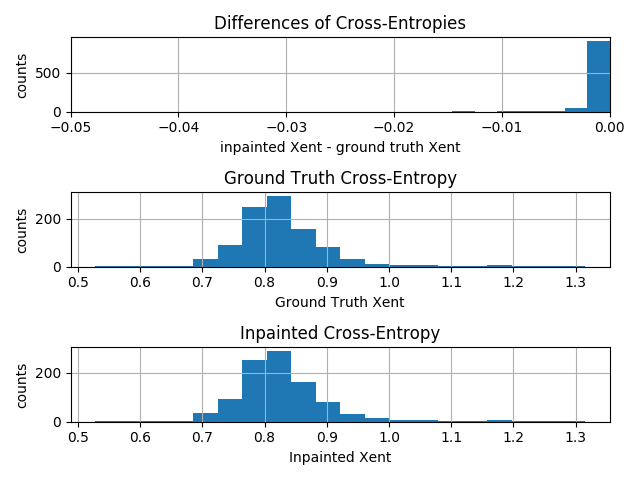
\includegraphics[width=1.0\textwidth]{task3/inpainting_1_hist.png}
      \caption{Cross entropy histograms, 1 pixel patch}
      \label{fig:Xent_hists_1}
    \end{figure}

    \begin{center}
      \begin{tabular}{ |c|c|c|c| } 
        \hline
        Cross entropy & Ground Truth & Inpaintings & Difference \\
        \hline
        Mean & 0.83094 & 0.82982 & -0.00112 \\
        Standard deviation & 0.08606 & 0.08436 & 0.00909 \\
        \hline
      \end{tabular}
    \end{center}

    \subsubsection{2x2 pixels inpainting}

    We have to following histograms of the cross-entropies over the 1000 images

    \begin{figure}[H]
      \centering
      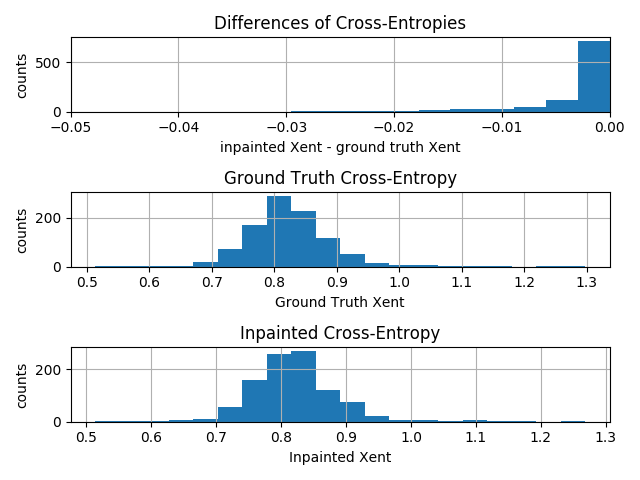
\includegraphics[width=1.0\textwidth]{task3/inpainting_2x2_hist.png}
      \caption{Cross entropy histograms, 2 by 2 pixel patch}
      \label{fig:Xent_hists_b2x2}
    \end{figure}

    \begin{center}
      \begin{tabular}{ |c|c|c|c| } 
        \hline
        Cross entropy & Ground Truth & Inpaintings & Difference \\
        \hline
        Mean & 0.82615 & 0.82206 & -0.00409 \\
        Standard deviation & 0.07245 & 0.06932 & 0.01523 \\
        \hline
      \end{tabular}
    \end{center}

    \subsubsection{Analysis}

    Comparing the histograms and cross entropy means and standard deviations we
    see that the difference in the cross entropy of the ground truth image and
    the optimal inpainted images are very low, majority of them between 0.001
    and 0 distance from each other. However, there are certain outliers (which
    still aren't very big, but further away than the bulk). I set the x-limit of
    the x-axis to be smaller so that the peak around 0 became more prominent,
    but meaning that a few outliers are outside the diagram for both 1 and 2 by
    2 pixel patches.

    The reason for why inpaintings always have a lower cross entropy than the
    ground truth is simple. As we test all of the different possible binary
    patches and taking the minimum as the inpainting, we will have that since
    the ground truth is equal to one of these patches that the cross entropy of
    the inpainting will be less or equal to the cross entropy of the ground
    truth. In reality, the in painting cross entropies that are far from the
    ground truth cross entropies reflect the shortcomings of the model.

    If we compare between the 1 pixel and 2 by 2 pixel patches we see that the 1
    pixel patch we see that the only real difference is that for just one pixel
    to inpaint, we get a zero difference much more often. This simply means that
    for fewer pixels, the model guess right more often as there are fewer
    combinations to actually guess (2 vs 16). This is reflected in the mean and
    standard deviation of the differences between the ground truth and inpainted
    cross entropy, where the mean is closer to 0 and standard deviation is
    smaller for the 1 pixel inpainting.

    \subsubsection{Example inpaintings}

    \begin{figure}[H]
      \centering
      \subfloat[1 Pixel patch inpainting]{
        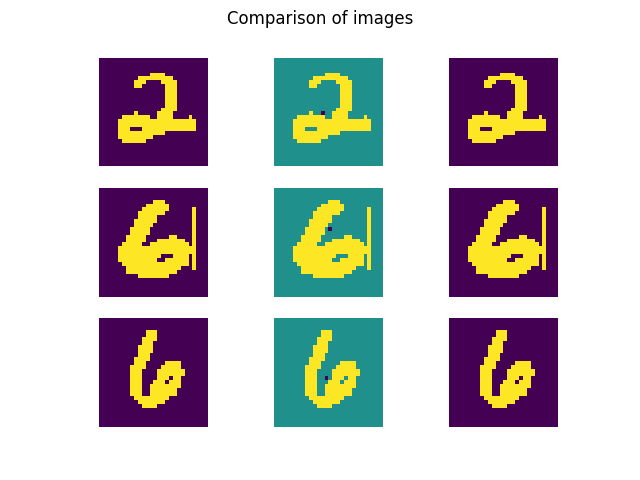
\includegraphics[width=65mm]{task3/image_comp_1pixel.png}
      }
      \subfloat[16 Pixel patch inpainting]{
        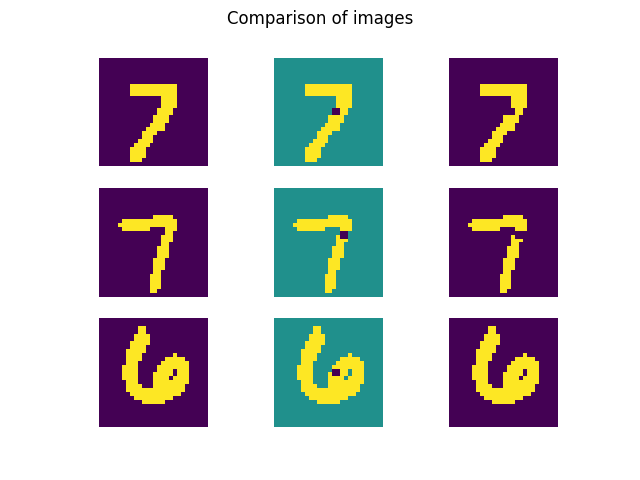
\includegraphics[width=65mm]{task3/image_comp_2x2pixel.png}
      }
      \caption{In order: Ground Truth, Masked, Inpainting. Rows specify index of
      image set.}
    \end{figure}

    \subsubsection{Saved .npy arrays}

    The saved inpaintings can be located in the directory relative to the parent
    directory, \\ \texttt{./code/data/inpainting\_data/}, and are called
    \\ \texttt{optimal\_inpaintings\_1pixel\_patch.npy} and \\ \texttt{optimal\_inpaintings\_2x2pixel\_patch.npy}.
    
\end{enumerate}

\newpage

\appendix

\section{task 2 images}

\subsection{generated images}

\subsubsection{ground truth and masked images}

\begin{figure}[H]
  \centering
  \subfloat[Ground truth]{
    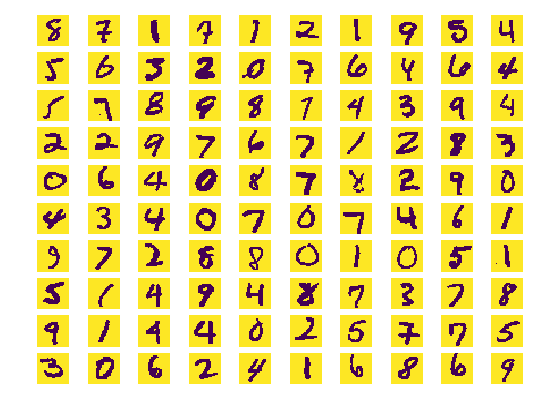
\includegraphics[width=65mm]{task2/gt_grid.png}
  }
  \subfloat[Masked]{
    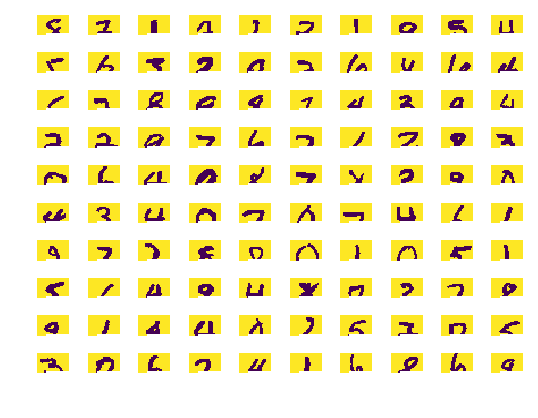
\includegraphics[width=65mm]{task2/masked_grid.png}
  }
  \caption{Ground truth and masked images sampled from the test set}
\end{figure}

\subsubsection{32 hidden units}

\begin{figure}[H]
  \centering
  \subfloat[1 pixel]{
    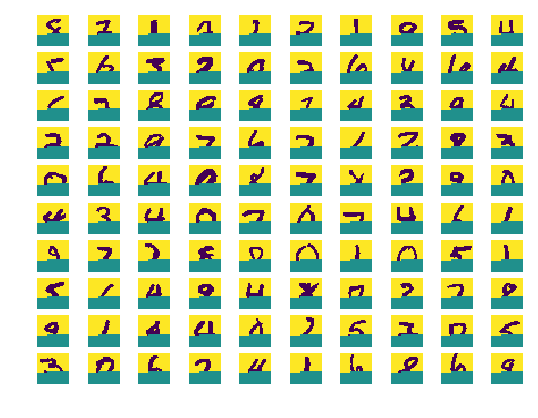
\includegraphics[width=65mm]{task2/task2b32pixels1/images/image_grid.png}
  }
  \subfloat[10 pixels]{
    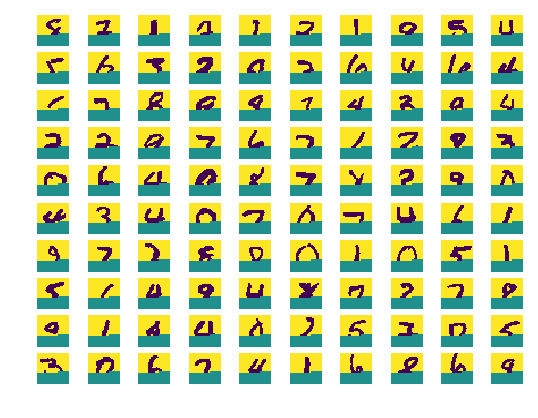
\includegraphics[width=65mm]{task2/task2b32pixels10/images/image_grid.png}
  }
  \hspace{0mm}
  \subfloat[28 pixels]{
    \includegraphics[width=65mm]{task2/task2b32pixels28/images/image_grid.png}
  }
  \subfloat[300 pixels]{
    \includegraphics[width=65mm]{task2/task2b32pixels300/images/image_grid.png}
  }
  \caption{first generated sample of each of the hundred test set images}
\end{figure}

\subsubsection{64 hidden units}

\begin{figure}[H]
  \centering
  \subfloat[1 pixel]{
    \includegraphics[width=65mm]{task2/task2b64pixels1/images/image_grid.png}
  }
  \subfloat[10 pixels]{
    \includegraphics[width=65mm]{task2/task2b64pixels10/images/image_grid.png}
  }
  \hspace{0mm}
  \subfloat[28 pixels]{
    \includegraphics[width=65mm]{task2/task2b64pixels28/images/image_grid.png}
  }
  \subfloat[300 pixels]{
    \includegraphics[width=65mm]{task2/task2b64pixels300/images/image_grid.png}
  }
  \caption{first generated sample of each of the hundred test set images}
\end{figure}

\subsubsection{128 hidden units}

\begin{figure}[H]
  \centering
  \subfloat[1 pixel]{
    \includegraphics[width=65mm]{task2/task2b128pixels1/images/image_grid.png}
  }
  \subfloat[10 pixels]{
    \includegraphics[width=65mm]{task2/task2b128pixels10/images/image_grid.png}
  }
  \hspace{0mm}
  \subfloat[28 pixels]{
    \includegraphics[width=65mm]{task2/task2b128pixels28/images/image_grid.png}
  }
  \subfloat[300 pixels]{
    \includegraphics[width=65mm]{task2/task2b128pixels300/images/image_grid.png}
  }
  \caption{first generated sample of each of the hundred test set images}
\end{figure}

\subsubsection{3 stacked layers of 32 hidden units}

\begin{figure}[H]
  \centering
  \subfloat[1 pixel]{
    \includegraphics[width=65mm]{task2/task2b32st3pixels1/images/image_grid.png}
  }
  \subfloat[10 pixels]{
    \includegraphics[width=65mm]{task2/task2b32st3pixels10/images/image_grid.png}
  }
  \hspace{0mm}
  \subfloat[28 pixels]{
    \includegraphics[width=65mm]{task2/task2b32st3pixels28/images/image_grid.png}
  }
  \subfloat[300 pixels]{
    \includegraphics[width=65mm]{task2/task2b32st3pixels300/images/image_grid.png}
  }
  \caption{first generated sample of each of the hundred test set images}
\end{figure}

\end{document}
